\subsection{Przykład}

\begin{frame}{Przykład}
  \centerline{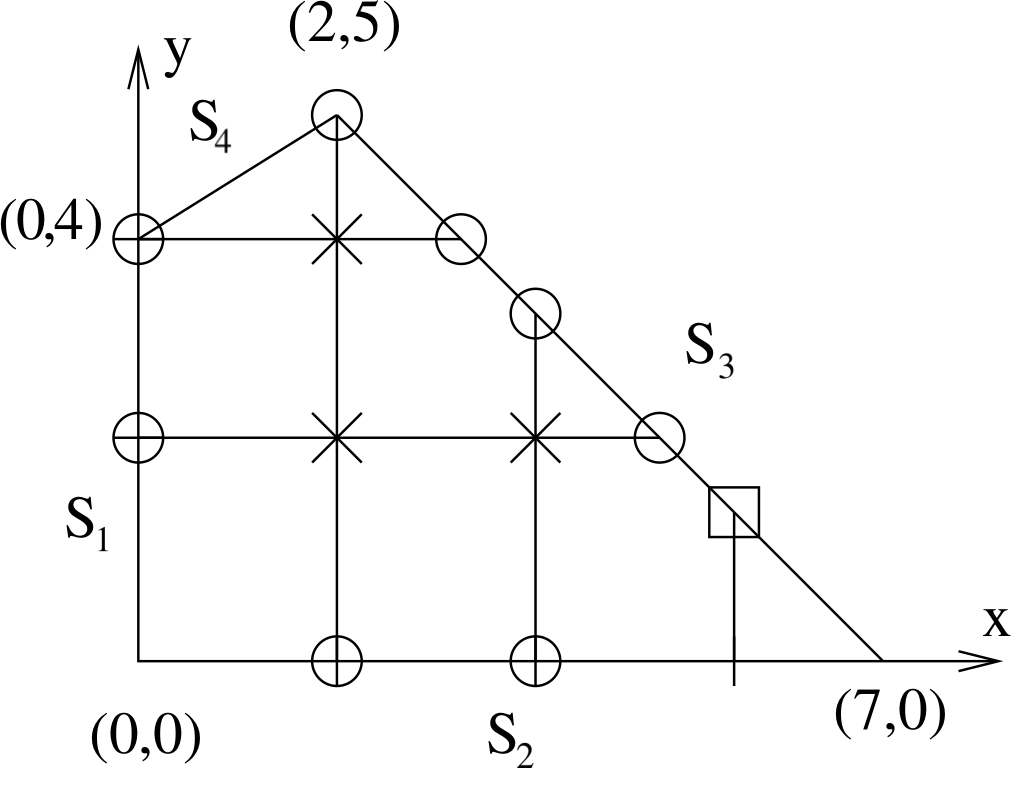
\includegraphics[height = 0.85 \textheight]{img/23/przyklad}}
\end{frame}

\begin{frame}
  \begin{block}{Oznaczenia}
    \begin{itemize}
      \item Czworokąt:
            $$(0,0), (7,0), (2,5), (0,4)$$
      \item $R$ -- wnętrze czworokąta
      \item $S$ -- brzeg czworokąta
      \item $S_i$, gdzie $i=1,\dots , 4$ -- boki czworokąta $\rightarrow$ brzeg $S$
    \end{itemize}
  \end{block}
\end{frame}

\begin{frame}
  Niech:
  \begin{itemize}
    \item $(\overline{x},\overline{y}) = (0,0);$
    \item $h=2$
  \end{itemize}

  Wówczas:
  \begin{itemize}
    \item Siatka wewnętrzna \begin{equation}R_h = \{(2,2),(2,4),(4,2)\} \end{equation}
    \item Punkty wspólne karty płaskiej i brzegu $S$: $S_h^* = S_i \bigcup S_2 \bigcup \text{(4 $\bigcirc$ i 1 $\square$ na $S_3$)}$ % CZY KWADRACIK TO POWINNA BYĆ *???
    \item Brzeg siatki:$$S_h = \{ (2,0),(4,0),(0,2),(5,2),(4,3),(3,4),(0,4),(2,5) \}\quad (\bigcirc)$$
  \end{itemize}
\end{frame}

\begin{frame}
  \begin{block}{Algorytm rozwiązywania zagadnienia Dirichleta}
    \begin{description}
      \item[krok 1]
        Dla ustalonych $h>0, (\overline{x},\overline{y})$
        \begin{itemize}
          \item tworzymy $R_h$ o $m$ punktach,
          \item tworzymy $S_h$ o $n$ punktach,
          \item numerujemy $R_h$ liczbami całkowitymi $[0,m]$ narastająco od lewej do prawej, z dołu do góry,
          \item numerujemy $S_h$ liczbami całkowitymi $[m+1, n+1]$ dowolnie.
        \end{itemize}
      \item[krok 2]
        W każdym $P_k(x,y) \in S_h$ podstawiamy $u_k = f(x,y)$.
    \end{description}
  \end{block}
\end{frame}

\begin{frame}
  \begin{block}{Algorytm rozwiązywania zagadnienia Dirichleta -- c.d.}
    \begin{description}
      \item[krok 3]
        W każdym $(x,y) \in R_h$ zapisujemy różnicowy odpowiednik równania Laplace'a:
        \begin{multline*}
          $$-2 \cdot ( \frac{1}{h_1 h_3} + \frac{1}{h_2 h_4}) \cdot u(x,y) + \\
          + \frac{2}{h_1 (h_1 + h_3)} u(x+h_1,y) + \frac{2}{h_2 (h_2 + h_4)} u(x,y + h_2) + \\
          + \frac{2}{h_3 (h_1 + h_s)} u(x-h_3,y)+\frac{2}{h_2 (h_2 + h_4)} u(x,y - h_4)=0$$ % 1. h_s W MIANOWNIOKU NIE MA ŻADNEGO SENSU (podejrzewam h_3)!!! 2. BARDZIEJ BYM SIĘ SPODZIEWAŁ h_4 PRZED NAWIASEM W MIANOWNIKU W OSTATNIM WYRAZIE
        \end{multline*}
        jeżeli zaś punktem sąsiednim $(x,y)$ jest punkt $\in S_{h^-}$ % CZYŻBY CHODZIŁO O S_h^* ???
        to $u$ w punkcie sąsiednim zastępujemy przez wartość $f(x,y) \rightarrow$ krok 2.

        Otrzymujemy układ $m$ równań o $m$ niewiadomych.
      \item[krok 4]
        Rozwiązanie układu równań.
    \end{description}
  \end{block}
\end{frame}

\begin{frame}
  \begin{block}{Algorytm rozwiązywania zagadnienia Dirichleta -- c.d.}
    \begin{description}
      \item[krok 5]
        Dyskretna funkcja $u_i$, gdzie $i=1,2, \dots ,m+n$, określona tylko na $R_h + S_h$, reprezentuje przybliżone rozwiązanie zagadnienia Dirichleta.
    \end{description}
  \end{block}

  \begin{block}{Stosowanie powyższego algorytmu opiera się na poniższych faktach}
    \begin{enumerate}
      \item przybliżone rozwiązanie zagadnienia Dirichleta istnieje i jest jednoznaczne,
      \item dla szerokiej klasy zagadnień rozwiązanie numeryczne jest zbieżne do analitycznego z $h \rightarrow 0$,
      \item otrzymany układ równań może być rozwiązany metodą SOR dla dowolnego przybliżenia początkowego z $ \omega \in (0,2)$; dla pewnych klas zagadnień można znaleźć optymalne wartości $\omega$ (najszybsza zbieżność procesu iteracyjnego).
    \end{enumerate}
  \end{block}
\end{frame}

\begin{frame}
  \begin{exampleblock}{Przykład}
    $S$: 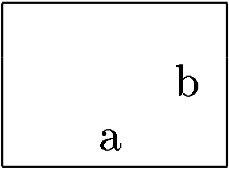
\includegraphics[width = 0.2 \textwidth]{img/23/prostokat}
    $$ \omega = \frac{2}{1 + \sqrt{1 - \lambda ^2}}, \quad \lambda = \frac{1}{2} \left( \cos \frac{\pi \cdot h}{a} + \cos \frac{\pi \cdot h}{b} \right)$$
  \end{exampleblock}

  \begin{alertblock}{Uwaga}
    Układ równań liniowych ma macierz diagonalnie dominującą $\Rightarrow$ wynik uporządkowania, określonego w kroku 3: na diagonali -- współczynniki przy $u(x,y)$.
  \end{alertblock}
\end{frame}

\begin{frame}
  \textit{Powrót do przykładu}

  \begin{itemize}
    \item $R$ -- wnętrze czworoboku
    \item $S$ -- bok czworoboku
    \item zagadnienie Dirichleta $z$
    \item $f(x,y) = x^2 - y^2$ na $S$
    \item $(\overline{x}, \overline{y}) = (0,0), h=2$
    \item $R_h$: $1,2,3$
    \item $S_h$: $4,5, \dots , 11$
  \end{itemize}
\end{frame}

\begin{frame}
  \centerline{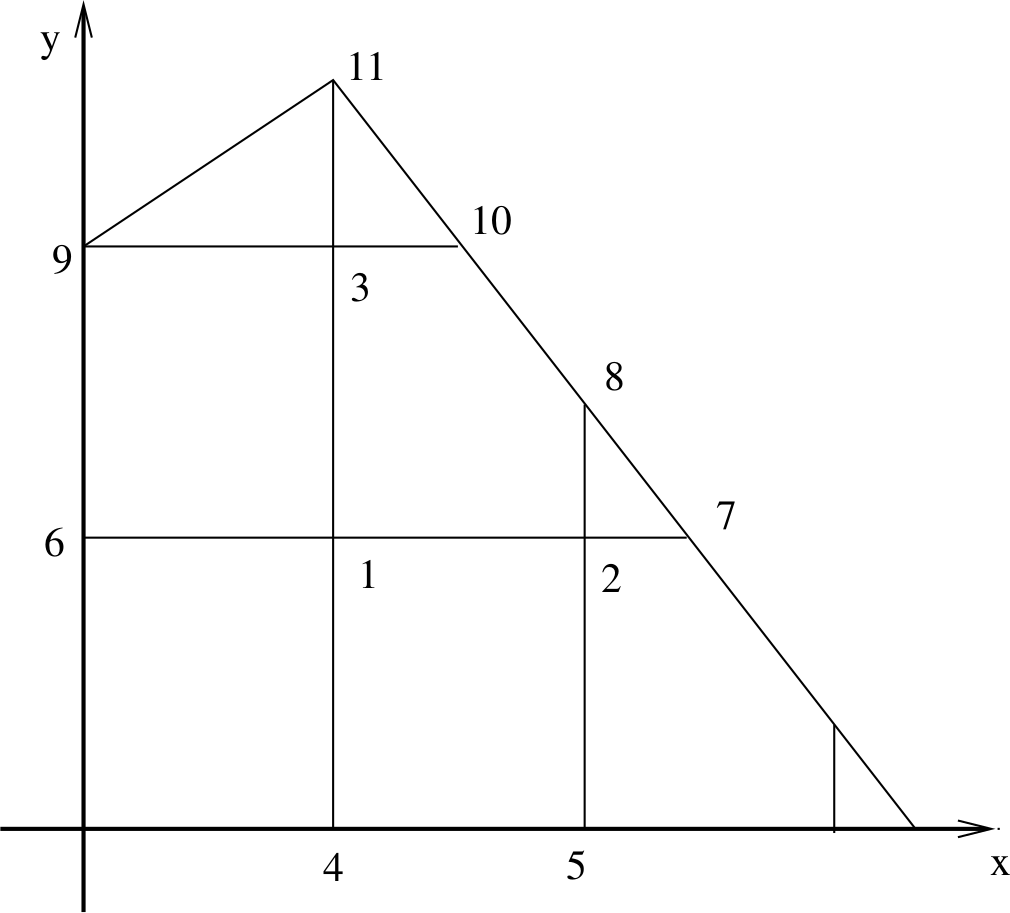
\includegraphics[height = 0.85 \textheight]{img/23/przyklad2}}
\end{frame}

\begin{frame}
  $$ u_4 = 4, u_5 = 16, u_6 = -4, u_7 = 21 $$
  $$ u_8 = 7, u_9 = -16, u_{10} = -7, u_{11} = -21 $$

  \begin{multline*}
    $$ -2 (\frac{1}{h_1 h_3} + \frac{1}{h_2 h_4}) u_0 + \\
    + \frac{2 u_1}{h_1 (h_1 + h_3)} + \frac{2 u_2}{h_2 (h_2 + h_4)} + \frac{2 u_3}{h_3 (h_1 + h_3)} + \frac{2 u_4}{h_4 (h_2 + h_4)} = 0 $$
  \end{multline*}
\end{frame}

\begin{frame}
    $$ \left\{ \begin{array}{ll}
    -u_1 + \frac{1}{4} u_2 + \frac{1}{4} u_3 + \frac{1}{4} (-4) + \frac{1}{4} \cdot 4 & =0 \\
    -2 u_2 + \frac{2}{3} \cdot 21 + \frac{2}{3} \cdot 7 + \frac{1}{3} u_1 + \frac{1}{3} \cdot 16 & =0 \\
    -2 u_3 + \frac{2}{3} (-7) + \frac{2}{3} (-21) + \frac{1}{3} (-16) + \frac{1}{3} u_1 & =0
    \end{array} \right. $$

  $$ \left\{ \begin{array}{llll}
  - u_1 & + \frac{1}{4} u_2 & +\frac{1}{4} u_3 & =0 \\
  \frac{1}{3} u_1 & -2 u_2 && =-24 \\
  \frac{1}{3} u_1 && -2 u_3 & =24
  \end{array} \right. $$

  Rozwiązanie: $u^T = (0, 12, -12)$.
\end{frame}
